\subsection{Know about}

The user will need to know that he has this resource and can use it because although we optimize the represantation of the
data set and we offer it to users, this will not be useful if users are not aware that it exists.

\subsubsection{How to solve it} 
The best way is to advertise the product in the right environment and environment.
\subsubsection{How we solve it. Aire Guru} 
Our tool is implemented for the city of Malaga, so we are currently working to give it to
know in this city.
It is currently available in the open data portal in the app tab \footnote {\url {https://datosabiertos.malaga.eu/aplicaciones}} \\
Participated in the first open data reuse contest organized by the Malaga City Council \footnote {\url {https://tinyurl.com/yx9wzutj}}
being finalist in the category of web page.


\begin{figure}[ht]
    \centering
   \subfigure[Advertising in the open data portal of Málaga]{ \centering 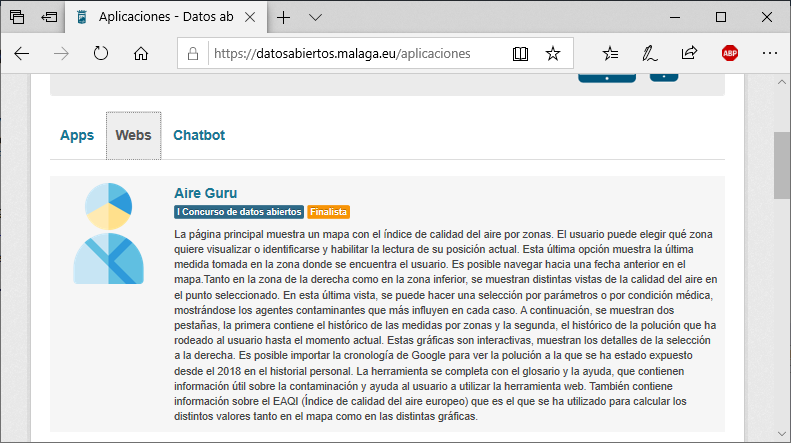
\includegraphics[width=6cm]{aireGuruFinalist}}
   \hfill
   \subfigure[Finalist]{ \centering 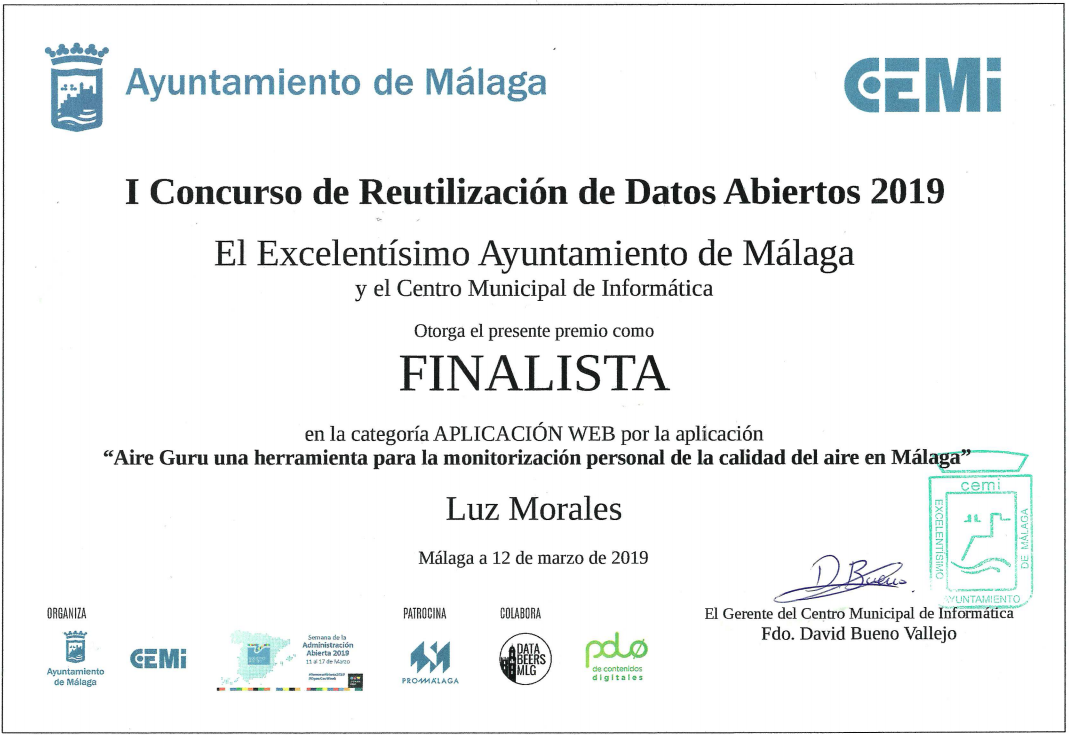
\includegraphics[width=5cm]{aireGuruFinalistCertificate}}
 
    \caption{I Contest of reuse of open data. Malaga's town hall}
    \end{figure}

\elsparagraph{Evaluation}  
\begin{itemize}
    \done It is currently published in the open data portal of the City of Malaga.
\crossed More work should be done on the advertising of the platform and make it known.
\end{itemize}
\newpage